\documentclass{article}

\usepackage[export]{adjustbox}
\usepackage{listings}
\usepackage{subcaption}
\usepackage{wrapfig}
\usepackage[dvipsnames]{xcolor}
\usepackage{float}
\usepackage{graphicx}
\usepackage[utf8]{inputenc}
\usepackage[a4paper, top=4cm, bottom=4cm, left=4cm, right=4cm]{geometry}

\title{
    \textbf{\textit{SafeStreets}} \\
    \textbf{DD document}}

\date{Academic year: 2019 - 2020}
\author{
    Dario Miceli Pranio \\
    Pierriccardo Olivieri
}

\begin{document}
\pagenumbering{gobble}

\maketitle

%%%%%%%%%% LOGO POLIMI %%%%%%%%%%
\begin{figure}[h!]
    \centering
    
\includegraphics[scale=0.5]{img/logo.png}
\end{figure}

\newpage
\pagenumbering{arabic}
\tableofcontents

\newpage
%%%%%%%%%% CHAPTER 1 %%%%%%%%%%
\section{Introduction}

\subsection{Purpose}
The purpose of this document is to provide a functional description of \textit{SafeStreets} application.

\subsection{Scope}
\textit{SafeStreets} is a service that aims to provide \textit{Users} with the possibility to notify \textit{Authorities} when traffic 
violations occur, and in particular parking violations. The application's goal is achieved by allowing \textit{Users} 
to share photo, position, date, time and type of violation and by enabling \textit{Authorities} to request them.
\\
\\
\textit{SafeStreets} requires the \textit{Users} to create an account to access its services, the functionalities unlocked after 
registration depend on the type of account created.
\\
If a \textit{User} creates an account as \textit{Citizen}, he/she must provide name, surname and a fiscal code in order to prove 
that he/she is a real person. Furthermore, he must provide an email with which he will be uniquely identified 
and a password. Once the account has been activated, \textit{User} can finally start to report parking violations and can also see 
statistics of the streets or the areas with the highest frequency of violations.
\\
\\
On the other hand, an officer will create an account as \textit{Authority} and he will need to provide his name, surname, 
work's Matricola, a password and as for \textit{Citizen}, will be uniquely identified by an email. Once the Matricola 
has been verified and the account has been activated, the officer can retrieve the potential parking violations 
sent by \textit{Citizen} that have not been taken into account yet by other officers, analyze them and, if it is the 
right case, generates traffic tickets. \textit{Authorities}, can see the same statistics of the \textit{Citizen} and can also see
statistics about vehicles' license plate that commit the most violations.


\subsection{Definitions, acronyms, abbreviations}

\subsubsection{Definitions}
\begin{itemize}
    \item \textit{Users}: can be either \textit{Citizen} or \textit{Authority}
    \item \textit{traffic violation}: generic violation that can occur in a street
    \item \textit{parking violation}: a violation caused by a bad parking
    \item \textit{violation}: general violation, identity both traffic or parking violation
    \item \textit{unsafe areas}: areas with an high rate of violations
\end{itemize}

\subsubsection{Acronyms}
Table with all acronyms used in document.
\begin{center}
\begin{tabular}{ | l | l |}
    \hline
    ACRONYM & COMPLETE NAME \\
    \hline
    DD & Design Document \\
    \hline
    RASD & Requirements Analysis and Specification Document \\
    \hline
    GPS & Global Positioning Systems \\
    \hline
    S2B & Software To Be \\
    \hline
    GDPR & General Data Protection Regulation \\
    \hline 
    FC & Fiscal Code \\
    \hline
    DB & Database \\
    \hline
\end{tabular}
\end{center}

\subsubsection{Abbreviations}
\begin{itemize}
    \item \textbf{Rn}: n-th Requirement 
\end{itemize}

\subsection{Revision History}

\subsection{Reference documents}
\begin{itemize}
    \item ISO/IEC/IEEE 29148: https://www.iso.org/standard/45171.html
    \item Specification Document: "SafeStreets Mandatory Project Assignement"
\end{itemize}

\subsection{Document Structure}
%%%%%%%%%% !CHAPTER 1 %%%%%%%%%%

\clearpage

%%%%%%%%%% CHAPTER 2 %%%%%%%%%%
\section{Architectural Design}

\subsection{Overview: High level components and their interaction}

\begin{figure}[H]
    \centering
    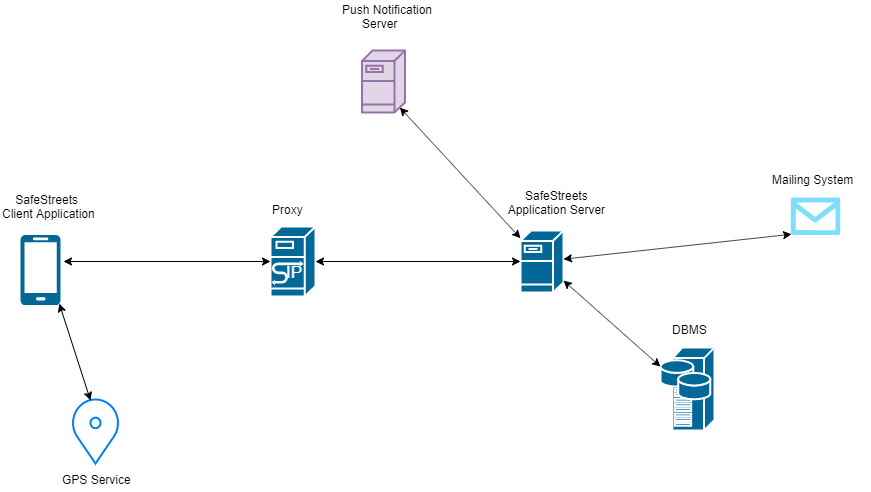
\includegraphics[scale=0.5]{img/Overview.png}
    \caption{\textit{System}'s Overview}
\end{figure}

In this graphical representation of \textit{SafeStreets} we describe at an high level the main interaction
between the components that are involved. Focusing on client side \textit{SafeStreets} provides a Client 
application, in this view case we don't make a distinciton between the \textit{Users} type, this is 
primarily devoted to the fact that the requests are similar. We identify then a 3-tier architecture, 
composed by the client, a proxy in the middle to manage properly all the requests and finally a back 
end part in which the \textit{System} store the information (in a DBMS) and generate statistics thanks
to the data submitted by the \textit{Citizen} and confirmed by \textit{Authorities}. In order to do this
we need an application server. Since we will authenticate the \textit{Users} through a confirmation email, 
and we give the possibility to the \textit{Authority} to receive data via mail, the \textit{System} needs
also a Mailing System. For notify the \textit{Users} with some relevant informations \textit{System} will 
use a notification System. Finally we also need some service in the client like GPS Service and Maps Service.


\subsection{Component view}

The purpose of this UML diagram is to show the internal architecture of the System's software. It's divided in 
three component: \textit{SafeStreets} Client Application, SafeStreets} Business Logic, External interfaces.
Below we will describe each component. 

\textbf{\textit{SafeStreets} Client Application} \\
This component is located on the \textit{User}'s device. Its modules are the Network Manager, the Presentation 
Component and Security Manager. The role of the first component is 
to dispatch all incoming and outgoing communications with the application server. The Presentation Component, 
instead, corresponds to the “View” in the MVCS Pattern.

\textbf{\textit{SafeStreets} Business Logic} \\
This component describes core logic of \textit{SafeStreets} application. It is a stateless module 
that lies between the Client application and the central Database. Now we will describe each component:
\begin{itemize}
    \item \textbf{Network Manager} \\
    It handles all incoming messages exchanged between Clients and Server. It does two foundamental
    things; it sends all incoming messages from client application to the correct handler in Business
    Logic and on the contrary it collects all the outgoing messages and sends to the corresponding Client
    Application.
    \item \textbf{Authentication Manager} \\
    The Authentication Manager exposes all methods related to the access to the platform. It handles the
    phase of \textit{User} registration and login and in order to do this it has to continuosly interact with 
    the database through the Data Storage Interface. It also checks all the costraints in order to garantee 
    creation of correct account. Furthermore it sends email to all the \textit{Users} that have been registered 
    by accessing the Mailing \textit{System}'s Interface. 
    \item \textbf{Citizen Manager} \\
    The \textit{Citizen} manager handles all functionalities related to a \textit{Citizen} Account. In order to
    do this it has to continuosly interact with database through the Data Storage Interface. It also allows
    \textit{Citizen} to update his setting. 
    \item \textbf{Authority Manager} \\
    The \textit{Authority} manager handles all functionalities related to an \textit{Authority} Account. In order to
    do this it has to continuosly interact with database through the Data Storage Interface. It also allows
    \textit{Authority} to update his setting.
    %%\item \textbf{Data Manager} \\
    %%This component is the main gateway between the Client Applications and the central Database. It handles the import of 
    %%new data associated to a \textit{User}'s account and its retrieval.
    %\item \textbf{Send Report Manager}\\
    %The Send Report Manager handles the creation and the management of a Send Report performed by \textit{Citizen} and
    %directed to \textit{System}. Inserting is possible thanks to Data Storage Manager. Furthermore, in order to avoid 
    %alteration, the Report is encrypted by using Privacy Manager.
    %\item \textbf{Retrieve Report Manager}\\
    %The Retrieve Report Manager handles the management of a Retrieve Report performed by \textit{Authority}. Retrieving 
    %is possible by querying the central Database through the Data Storage Interface.
    \item \textbf{Statistics Manager} \\
    The Statistics Manager handles the management of a Retrieve Statistics performed by \textit{User}. Retrieving 
    is possible by querying the central Database through the Data Storage Interface.     
    \item \textbf{Privacy Manager} \\
    The Privacy Manager exposes methods to encrypt sensitive data. This operation is important in order to avoid data leaks
    and data alteration.
    \item \textbf{Data Storage Manager} \\
    The Data Storage Manager provides all methods to interact with the central Database such as data retrieval, 
    storage and update.
    
\end{itemize}

\textbf{External interfaces} \\
Some of the described components in our \textit{System} are also dedicated to communicating with external services through 
specific interfaces. It is essential that the communication works properly in order to fulfill application's functionalities.
This external services are:
\begin{itemize}
    \item Database \\
    The component devoted to interacting with the central database on cloud is the Data Storage Manager.
    \item GPS \\
    On the Client side of the application, \textit{SafeStreets} access data from the \textit{User}'s device's GPS through
    the Data Manager Interface. GPS information are important because are used in report to locate a position. 
    \item Mailing System \\
    It used by Authentication Manager to inform an \textit{User} that his account has been correctly created. 
    \item Maps Service \\ 
    It's used to show unsafe areas in statistics.  
\end{itemize}  

\subsection{Deployement view}
\begin{figure}[H]
    \centering
    \includegraphics[scale=0.5]{img/Deployement_component.png}
    \caption{Deployment view}
\end{figure}  
The architecture choosed for \textit{SafeStreets} is a multi-tier architecture. Below all the nodes 
involved will be described.
\\
\\
\textbf{Smarthphone}\\
Represents the \textit{User's} smarthphone in which the client will run. This is the client machine
that will run \textit{SafeStreets} application.
\\
\\
\textbf{Firewall}\\
Necessary to provide protection between local network and world network, so not-allowed third parties will not be 
able to access data. In particular we decided to use two firewalls to create a DMZ. The first firewall must be configured 
to allow traffic destined to the DMZ only. The second firewall only allows traffic to the DMZ from the internal network.
\\
\\
\textbf{Application Server}
Is the central unit of \textit{SafeStreet} all the other components refer to this. It contains all
the logic and provide bidirectional access to Database i.e. manages data acquisition and requests.
Since for \textit{SafeStreet} we need to focus on security, is a though decision to have only one main
unit.
\\
\\
\textbf{Proxy}
\textit{System} will use a web server to receive requests. This solution is more scalable for the eventuality
of further improvements and guarantee a better stability of the \textit{System}.  
\\
\\
\textbf{Database}\\
A Database is necessary in order to store all the informations about personal data, registration and 
data submitted by \textit{Citizen} and retrieve information in order, for instance, to build statistics.

\section{User Interface Design} 
\section{Requirements Traceability}
\begin{center}
    \begin{tabular}{ | l | l |}
        \hline
        COMPONENT(DD) & REQUIREMENTS(RASD) \\
        \hline
        Authentication Manager & [R1]: Account can be created if and only if User provides unique email and password \\
                               & [R2]: The System allow Guest to create Citizen or Authority account \\
        \hline
        Citizen Manager & [R3]: The Citizen has to take the violation’s photo with the application \\
                        & [R4]: The System allows Citizen to input some violation’s data \\
                        & [R5]: The photo taken must be recognizable by the System \\
                        & [R6]: The Citizen has to be able to discard the photo taken \\
                        & [R7]: The System has to be able to attach the correct date, time and position to the report \\
                        & [R8]: The Citizen can’t change date, time and position in the report \\ 
                        & [R9]: Citizen can change the license plate if it isn’t recognised properly \\
                        & [R10]: Citizen has to be able to choose the correct type of violation \\ 
        \hline
        %%vanno messi R11, 12, 14???
        Authority Manager & [R17]: The violation retrieved can only be seen by the Authority that retrieves it \\
                          & [R13]: Authority can search for a specific license plate \\
        \hline
        Statistics Manager & [R11]: Users can change the area of visualization \\
                           & [R12]: Users can change the date of visualization \\
                           & [R13]: Authority can search for a specific license plate \\
                           & [R14]: Users can change the date of visualization \\
                           & [R18]: The System must update the statistics with the most recent data \\
        \hline
        Privacy Manager & [R16]: The System must use HTTPS to safely communicate \\
        %%come il network manager probabilmente si può evitare
        %%\hline 
        %%Data Storage Manager &  \\
        \hline
        Security Manager & [R15]: Violations sent must be digitally signed and hashed \\
                         & [R16]: The System must use HTTPS to safely communicate \\
        \hline
    \end{tabular}
    \end{center}


\end{document}